\documentclass[a4paper,11pt]{article}

\usepackage[T1]{fontenc}
\usepackage[utf8]{inputenc}
\usepackage{graphicx}
\usepackage{xcolor}

\renewcommand\familydefault{\sfdefault}
\usepackage{tgheros}
\usepackage[defaultmono]{droidmono}

\usepackage{amsmath,amssymb,amsthm,textcomp}
\usepackage{enumerate}
\usepackage{multicol}
\usepackage{tikz}
\usepackage{graphics}
\usepackage{lstlinebgrd}
\usepackage{color}
\usepackage{geometry}
\geometry{total={210mm,297mm},
left=25mm,right=25mm,%
bindingoffset=0mm, top=20mm,bottom=20mm}


\linespread{1.3}

\newcommand{\linia}{\rule{\linewidth}{0.5pt}}

\newtheoremstyle{mytheor}
    {1ex}{1ex}{\normalfont}{0pt}{\scshape}{.}{1ex}
    {{\thmname{#1 }}{\thmnumber{#2}}{\thmnote{ (#3)}}}

\theoremstyle{mytheor}
\newtheorem{defi}{Definition}

% my own titles
\makeatletter
\renewcommand{\maketitle}{
\begin{center}
\vspace{2ex}
{\huge \textsc{\@title}}
\vspace{1ex}
\\
\linia\\
\@author \hfill \@date
\vspace{4ex}
\end{center}
}
\makeatother
%%%

% custom footers and headers
\usepackage{fancyhdr}
\pagestyle{fancy}
\lhead{Page \thepage}
\chead{}
\rhead{Steven Seppala}
\lfoot{Programming assignment \textnumero{} 5}
\cfoot{Operating Systems}
\rfoot{ECE 437}
\renewcommand{\headrulewidth}{0pt}
\renewcommand{\footrulewidth}{0pt}
%

% code listing settings
\usepackage{listings}
\lstset{
    language=[ANSI]C,
    basicstyle=\ttfamily\small,
    aboveskip={1.0\baselineskip},
    belowskip={1.0\baselineskip},
    columns=fixed,
    extendedchars=true,
    breaklines=true,
    tabsize=4,
    prebreak=\raisebox{0ex}[0ex][0ex]{\ensuremath{\hookleftarrow}},
    frame=lines,
    showtabs=false,
    showspaces=false,
    showstringspaces=false,
    keywordstyle=\color[rgb]{0.627,0.126,0.941},
    commentstyle=\color[rgb]{0.133,0.545,0.133},
    stringstyle=\color[rgb]{01,0,0},
    numbers=left,
    numberstyle=\small,
    stepnumber=1,
    numbersep=10pt,
    captionpos=t,
    escapeinside={\%*}{*)}
}
	\definecolor{dkgreen}{rgb}{0,0.8,0}
	\definecolor{gray}{rgb}{0.5,0.5,0.5}
	\definecolor{mauve}{rgb}{0.58,0,0.82}

%%%----------%%%----------%%%----------%%%----------%%%
%%%----------Document begins right below this-------%%%
%%%----------%%%----------%%%----------%%%----------%%%
\begin{document}

\title{Homework Assignment \textnumero{} 2}

\author{Steven Seppala}

\date{26 October 2014}

\maketitle

\begin{center} \section*{Homework assignment 2} \end{center}

\begin{enumerate}
\item {Problem 6.14} 
    \par \emph{(A)} With $\alpha$ and $\tau _{0}$ both equal to zero. This will imply $\tau _{n+1}$ = $\tau _{0}$ = 100 ms. This therefor implies that the recent history has no effect and that the formula will always predict 100 ms for the next CPU burst.
    \par \emph{(B)} The most recent behavior of the process is given much higher weight than the past estimated value. Consequently, the scheduling algorithm is almost memory-less, and simply predicts the length of the previous burst for the next quantum of CPU execution.
    
\item {Problem 6.16}
    \par 
    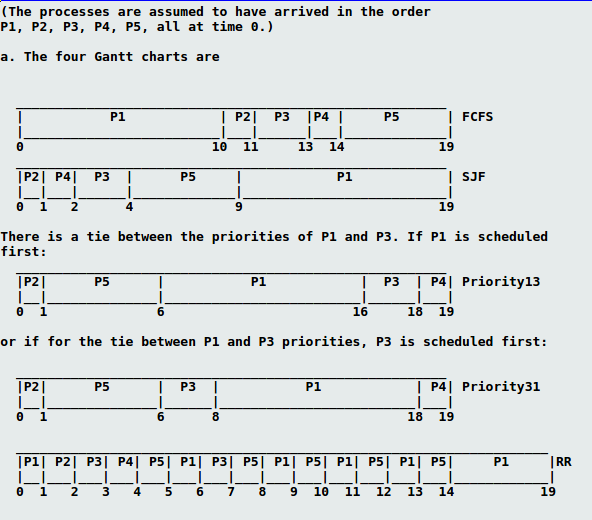
\includegraphics[width=1\textwidth]{q2}
    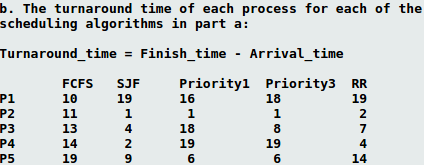
\includegraphics[width=1\textwidth]{q2b}
    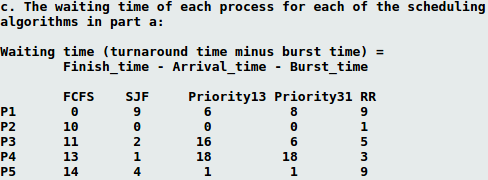
\includegraphics[width=1\textwidth]{q2c}
    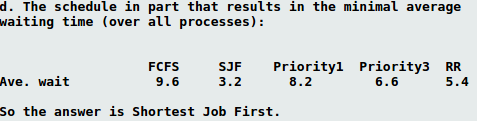
\includegraphics[width=1\textwidth]{q2d}
    \pagebreak
\item{Problem 6.23}
    \par With $\beta$ $\textgreater$ $\alpha$ $\textgreater$ $0$ ; this implies a FIFO. 
    \par With $\beta$ $\textgreater$ $\alpha$ $\textgreater$ $0$ ; this implies a LIFO. 

\item {Ch 6. About UNIX scheduling}
    \par 
    Given that base = 60: \\
    P_{1} = \frac{40}{2} $+ 60$ = $80$ \\
    P_{2} = \frac{18}{2} $+ 60$ = $69$ \\
    P_{3} = \frac{10}{2} $+ 60$ = $65$ \\
    \par Thus the new priorities are : $P_{3}$  first $P_{2}$ second, and then $P_{1}$ last.
    
\setlength\parindent{24pt}

\item {Problem 5.23}\\
1.Initialize semaphore to $MAX\_SOCKETS$ \\
2.A new incoming connection will wait() on the semaphore
\par a.If the semaphore's value is less than 0, block
\par b.If the semaphore's value is greater than or equal to 0, accept connection\\
3.When a connection is closed, signal() the semaphore\\
4.Go back to 2 for possible new connections\\
\pagebreak
\item {Problem 5.23}
    \par 
    \lstinputlisting[basicstyle=\small]{sudo-code.c}
    
\item {Problem 5.17}
    \par For a short duration lock, it would be better to use a spinlock.\\
    If the lock is going to be held for a long time, it should be a mutex lock which blocks while it sleeps waiting for it to become available. \\
    If a thread may be put to sleep while holding the lock, it is better to use a mutex lock so that another thread may not be accidentally allowed into the sensitive code.

\pagebreak
\item {Problem 7.16}
    \par 
    \begin{enumerate}
    \item Safe anytime.
    \item Safe only when Max $\leq$ Available.
    \item Safe only when Max $\leq$ Available.
    \item Safe anytime.
    \item Safe anytime.
    \item Safe anytime.
    \end{enumerate}
\item{Problem 7.17}    
    \par 
    Proof by contradiction:\\
    Suppose the system is deadlocked. This implies that each process is holding one resource and is waiting for one more. Since there are three processes and four resources, one process must be able to obtain two resources. This process requires no more resources and, therefore it will return its resources when done. 

\item{Problem 7.23}
    \begin{enumerate}
    \item The values of Need for processes P$_0$ through P$_4$ respectively are: 
    \\(0, 0, 0, 0), (0, 7, 5, 0),  (1,0, 0, 2), (0, 0, 2, 0), and (0, 6, 4, 2). 
    
    \item Yes. With Available being equal to (1,5, 2, 0), either process P$_0$ or P$_3$ could run. Once process P$_3$ runs, it releases its resources, which allow all other existing processes to run. 

    \item Yes, it can. This results in the value of Available being (1, 1, 0, 0). One ordering of processes that can finish is P$_0$, P$_2$, P$_3$, P$_1$, and P$_4$. 

    \end{enumerate}
    

\end{enumerate}

\end{document}
